\documentclass{article}
\usepackage[utf8]{inputenc}
\usepackage{tikz, amsmath, amsthm, amssymb}
\newtheorem{thm}{Theorem}
\newtheorem{cor}{Corollary}
\newtheorem{lem}{Lemma}
\newtheorem{dfn}{Definition}

\tikzset{every picture/.style={line width=0.75pt}} %set default line width to 0.75pt

\title{Dynamical systems}
\author{Harambe}
\date{June 2020}

\begin{document}

\maketitle

\section{Case III: $\lambda^r=1$}

We will now start studying the case where $\lambda$ is a root of unity, i.e. $\lambda^r=1$ for rational (or equivalently, integer) $r$ (which we will see is qualitatively different from the irrational case) -- we call $z=0$ a \textit{parabolic fixed point}. Where $p+1$ is the smallest integer greater than 1 such that $z^{p+1}$ has a non-zero coefficient: 

\begin{equation}
    \label{eq:f}
    f(z) = \lambda z + \mu z^{p + 1} + o(z^{p+1})
\end{equation}

In order to characterize the attractive/repulsive nature of the fixed point, we are first interested in finding the \textit{attraction/repulsuion directions} to a fixed point. These are somewhat analogous to eigenvectors of linear transformations, but exhibit much richer behavior.

\subsection{Case IIIa: $\lambda = 1$}
The multiplier = +1 case appears to be simpler, as it is ``irrotational'' in some sense: the function appears to be the identity near the fixed point. In this case, $p+1$ is also called the \textit{multiplicity} of the fixed point, as it is the multiplicity of the $z=0$ root of $f(z)-z$.

We will first intuitively ponder about the nature of the fixed point in this case, and then formalize our results in Theorem~\ref{thm:arvec-ir}.

\begin{itemize}
    \item Consider infinitesimal complex $\varepsilon$ such that $f(\varepsilon)=\alpha\varepsilon$ for positive real $\alpha$ a function of $\varepsilon$ ($\forall \varepsilon, \alpha > 1$ corresponding to repulsion; $\forall \varepsilon, \alpha > 1$ corresponding to attraction). Substituting in Eq.~\ref{eq:f} to $p+1$ order in $z$ with $\lambda=1$:
    \begin{equation*}
        {\varepsilon^p} = (\alpha  - 1)/\mu 
    \end{equation*} 
    We can see that there are $p$ \textit{attraction vectors}, which correspond to the argument of $\varepsilon$ when $\alpha < 1$, and $p$ \textit{repulsion vectors}, which correspond to the argument of $\varepsilon$ when $\alpha > 1$. 
    \begin{equation*}
        \begin{array}{*{20}{c}}
            {v_ - ^p =  - 1/(p \mu) } \\
            {v_ + ^p =  + 1/(p \mu) }
        \end{array}    
    \end{equation*}
    (The reason for using $1/(p \mu)$ over $1/\mu$ is not important, and will become clear later.)
    Alternatively we may write, where $v_0$ is some repulsion vector, that $v_j$, defined as below, is attractive for odd $j$ and repulsive for even $j$: 
    \begin{equation}
        \label{eq:v}
        v_j = v_0 \exp\left(j/ p \cdot \pi i\right)
    \end{equation}
    \item We may also be interested in asking about the \textit{rate} of convergence of the iteration. Since $\lim_{\varepsilon\to 0}\alpha(\varepsilon) = 1$, which means the convergence is slower than exponential -- in addition, the convergence is slower for larger $p$. We may guess that the sequence $f^n(z)$ converges $\propto v_-/n^{1/p}$.
    \item Taking a cue from the nature of linear dynamical systems, we might imagine the local behavior of the iterated map to be something like that shown in Fig.~\ref{fig:basins}: that the sectors between consecutive repulsion vectors define \textit{attraction basins} for the attraction vector between them -- this would also imply that there are no small cycles near a parabolic fixed point.
\end{itemize}

\begin{figure}
    \label{fig:basins}
    \centering
    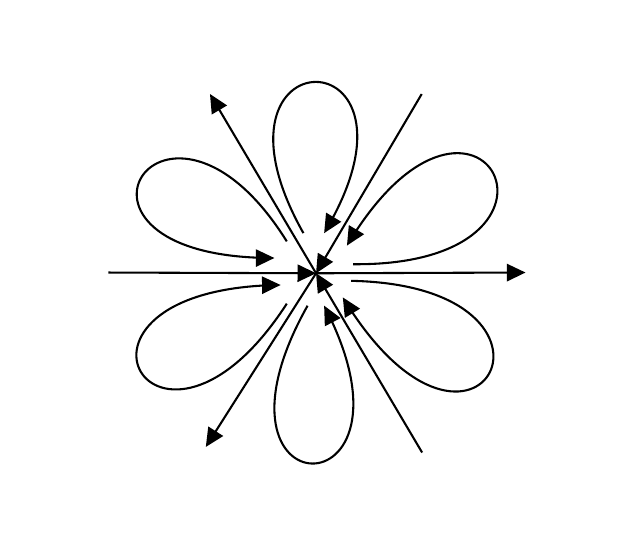
\begin{tikzpicture}[x=0.75pt,y=0.75pt,yscale=-1,xscale=1]
%uncomment if require: \path (0,235); %set diagram left start at 0, and has height of 235

%Straight Lines [id:da7014467597216401] 
\draw    (334,128.64) -- (431.9,128.29) ;
\draw [shift={(434.9,128.28)}, rotate = 539.79] [fill={rgb, 255:red, 0; green, 0; blue, 0 }  ][line width=0.08]  [draw opacity=0] (8.93,-4.29) -- (0,0) -- (8.93,4.29) -- cycle    ;
%Straight Lines [id:da7937079638414151] 
\draw    (334,128.64) -- (284.43,44.86) ;
\draw [shift={(282.9,42.28)}, rotate = 419.39] [fill={rgb, 255:red, 0; green, 0; blue, 0 }  ][line width=0.08]  [draw opacity=0] (8.93,-4.29) -- (0,0) -- (8.93,4.29) -- cycle    ;
%Straight Lines [id:da5652322657720215] 
\draw    (334,128.64) -- (282.51,209.74) ;
\draw [shift={(280.9,212.28)}, rotate = 302.40999999999997] [fill={rgb, 255:red, 0; green, 0; blue, 0 }  ][line width=0.08]  [draw opacity=0] (8.93,-4.29) -- (0,0) -- (8.93,4.29) -- cycle    ;
%Straight Lines [id:da49795176320656886] 
\draw    (384.9,42.28) -- (335.52,126.05) ;
\draw [shift={(334,128.64)}, rotate = 300.51] [fill={rgb, 255:red, 0; green, 0; blue, 0 }  ][line width=0.08]  [draw opacity=0] (8.93,-4.29) -- (0,0) -- (8.93,4.29) -- cycle    ;
%Straight Lines [id:da9443327330326834] 
\draw    (233.9,128.28) -- (331,128.63) ;
\draw [shift={(334,128.64)}, rotate = 180.21] [fill={rgb, 255:red, 0; green, 0; blue, 0 }  ][line width=0.08]  [draw opacity=0] (8.93,-4.29) -- (0,0) -- (8.93,4.29) -- cycle    ;
%Straight Lines [id:da7066291127526734] 
\draw    (385.1,215) -- (335.53,131.22) ;
\draw [shift={(334,128.64)}, rotate = 419.39] [fill={rgb, 255:red, 0; green, 0; blue, 0 }  ][line width=0.08]  [draw opacity=0] (8.93,-4.29) -- (0,0) -- (8.93,4.29) -- cycle    ;
%Curve Lines [id:da8961728852679585] 
\draw    (351.9,124.28) .. controls (472.29,125.27) and (412.51,10.81) .. (349.84,113.71) ;
\draw [shift={(348.9,115.28)}, rotate = 300.82] [fill={rgb, 255:red, 0; green, 0; blue, 0 }  ][line width=0.08]  [draw opacity=0] (8.93,-4.29) -- (0,0) -- (8.93,4.29) -- cycle    ;
%Curve Lines [id:da6878104068351576] 
\draw    (327.9,109.28) .. controls (273.17,12.15) and (394.67,12.65) .. (338.76,107.83) ;
\draw [shift={(337.9,109.28)}, rotate = 300.98] [fill={rgb, 255:red, 0; green, 0; blue, 0 }  ][line width=0.08]  [draw opacity=0] (8.93,-4.29) -- (0,0) -- (8.93,4.29) -- cycle    ;
%Curve Lines [id:da6213553894464128] 
\draw    (319.9,113.28) .. controls (261.19,19.13) and (195.56,120.63) .. (312.13,121.27) ;
\draw [shift={(313.9,121.28)}, rotate = 539.81] [fill={rgb, 255:red, 0; green, 0; blue, 0 }  ][line width=0.08]  [draw opacity=0] (8.93,-4.29) -- (0,0) -- (8.93,4.29) -- cycle    ;
%Curve Lines [id:da5023612601796306] 
\draw    (319.9,143.28) .. controls (257.21,240.17) and (196.51,136.7) .. (315.1,134.3) ;
\draw [shift={(316.9,134.28)}, rotate = 539.3399999999999] [fill={rgb, 255:red, 0; green, 0; blue, 0 }  ][line width=0.08]  [draw opacity=0] (8.93,-4.29) -- (0,0) -- (8.93,4.29) -- cycle    ;
%Curve Lines [id:da5020349766396639] 
\draw    (329.9,144.28) .. controls (273.18,245.15) and (389.72,245.66) .. (338.68,145.79) ;
\draw [shift={(337.9,144.28)}, rotate = 422.4] [fill={rgb, 255:red, 0; green, 0; blue, 0 }  ][line width=0.08]  [draw opacity=0] (8.93,-4.29) -- (0,0) -- (8.93,4.29) -- cycle    ;
%Curve Lines [id:da4534345213536044] 
\draw    (350.9,132.28) .. controls (469.3,134.65) and (411.49,244.55) .. (347.86,141.84) ;
\draw [shift={(346.9,140.28)}, rotate = 418.73] [fill={rgb, 255:red, 0; green, 0; blue, 0 }  ][line width=0.08]  [draw opacity=0] (8.93,-4.29) -- (0,0) -- (8.93,4.29) -- cycle    ;
\end{tikzpicture}

    \caption{Attraction and repulsion vectors, basins where $p = 3$, $\mu\in\mathbb{R}^{> 0}$}
\end{figure}

\begin{thm}
    \label{thm:arvec-ir}
    Let $f$ be a holomorphic function as in Eq.~\ref{eq:f} with $\lambda = 1$. Let $z_0$ be such that the sequence $z_n=f^n(z_0)\to 0$ but $\forall n, z_n\ne 0$. Then, for some attraction vector $v_j$ as defined as in Eq.~\ref{eq:v},
    \begin{equation*}
        \lim_{n\to\infty} n^{1/p} z_n = v_j
    \end{equation*}
    i.e. $z_n\sim v_j/n^{1/p}$ asymptotically. $z_n$ is said to tend to 0 in the direction of $v_j$.
\end{thm}
\begin{proof}
    The proof relies on a variable substitution $\omega(z)=-1/(p \mu z^p)$, $w_n=\omega(z_n)$. Although the substitution is not injective on all of $\mathbb{C}^{\times}$, one may define $2p$ restrictions of the function, $\omega_j(z):\Delta_j\to\mathbb{C}-\mathbb{R}_{(-1)^j}$, where $\Delta_j=\{re^{i\theta}v_j : r>0, |\theta| < \pi/p \}$. Then consider the map $\hat{f}_j(w):=\omega_j \circ f \circ \omega_j^{-1}(w)$, defined outside a large disk on $\mathbb{C}-\mathbb{R}_{(-1)^k}$ -- whose power series it is easy to compute:
    \begin{equation}
        \label{eq:fhat}
        \hat{f}_j(w) = w + 1 + o(1)
    \end{equation}
    Then clearly $w_n\sim n$ as $n\to\infty$ (formally: $w_{n+1}-w_n\to 1$, hence the partial sum $(w_n-w_0)/n\to 1$), which implies 
    \begin{equation}
        \label{eq:zp}
        z_n^p\sim -1/(p\mu n)
    \end{equation}
    Further, from Eq.~\ref{eq:fhat}, $\exists R > 0, \mathrm{Re}(w)>R \implies |\hat{f}_j(w)-(w+1)|<1/2$. Then $\hat{\mathcal{P}}:=\{w\mid\mathrm{Re}(w)>R\}$ is closed under $\hat{f}_j$, and the \textit{attracting petal} $\mathcal{P}_j=\omega_j^{-1}\left(\hat{\mathcal{P}}\right)$ is closed under $f$. Now since $\exists m, \mathrm{Re}(w_m)>R$, we must have $z_m\in \mathcal{P}_j$ for some $j$, and by closure of the attracting petal, all further $z_k$ are in this petal. Since by definition $\mathcal{P}_j\subseteq\Delta_j$, this means $z_n$ is eventually in $\Delta_j$, and we can take the $n$th root of Eq.~\ref{eq:zp}:
    \begin{equation}
        \label{eq:z}
        z_n \sim v_j/n^{1/p}
    \end{equation}
\end{proof}
\begin{cor}
    \label{cor:arvec-ir-inv}
    Let $z_0$ be such that the sequence $z_n=f^{-n}(z_0)\to 0$ but $\forall n, z_n\ne 0$. Then, for some repulsion vector $v_j$ of $f$ as defined in Eq.~\ref{eq:v}, $z_n\sim v_j/n^{1/p}$.
\end{cor}

\subsection{Case IIIb: $\lambda = \exp(q/r \cdot 2\pi i)$}
Once again, consider $f$ as in Eq.~\ref{eq:f}, but with $\lambda$ any primitive $r$th root of unity. Then near its fixed point $z=0$, $f(z)\approx \lambda z$, which for $\lambda\ne 1$ does not have ``true'' attraction and repulsion vectors in the sense that we have been imagining them. 

Instead, we define attraction and repulsion vectors in a way that is more analogous to the notion of limit points, in that we are satisfied with being asymptotic to subsequences.

\begin{dfn}
   Let $v$ be a complex number. 
    \begin{itemize}
        \item If there exists a sequence $z_n=f^n(z_0)\to 0$ with a subsequence $z_{n_k}$ such that $\arg z_{n_k}\to\arg v$, then $v$ is called an attraction vector for $f$.
        \item If there exists a seuqnece $z_n=f^{-n}(z_0)\to 0$ with subsequence $z_{n_k}$ such that $\arg z_{n_k}\to\arg v$, then $v$ is called an repulsion vector for $f$.
    \end{itemize}
\end{dfn}
\begin{thm}
    \label{thm:arvec-rot}    
    The attraction vectors of $f$ are the same as the same as those of $f^r$, and their number is a multiple of $r$.
\end{thm}
\begin{proof}
    Any sequence $z_n=f^n(z_0)\to 0$ can be partitioned into subsequences $z_{kr+s}$ for $s=0,\dots r-1$. Each subsequence is an orbit under $f^r$, which is a function of the form discussed in IIIa, thus the attraction vectors of $f$ are precisely those of $f^r$. For each $v$ asymptotic to $z_{kr}$, $\lambda^s v$ is asymptotic to $z_{kr+s}$. Thus any $z_n\to 0$ gives rise to $r$ attraction vectors for $f$. 
\end{proof}
\begin{cor}
    \label{thm:rot-mult}
    The multiplicity of the $z=0$ root of $f^r$ is congruent to 1 mod $r$. 
\end{cor}
Theorem~\ref{thm:arvec-rot} is crucial, as it allows us to often reduce problems about parabolic points to the case IIIa. We will be making this WLOG assumption about $f$ in sections that follow, and the general case will follow easily through Theorem~\ref{thm:arvec-rot}.

\subsection{Petals and basins}
The following definitions will help us in understanding the nature of the Fatou and Julia sets corresponding of the function $f$. 
\begin{dfn}
    \label{def:basin}
    The basin of attraction $\mathcal{B}_v$ for $v$ is defined as the set of points $z$ such that $f^n(z)\to 0$ in the direction of $v$. The immediate basin of attraction $\mathcal{B}_v^0$ is defined as the unique connected component of $\mathcal{B}_v$ that is closed under $f$.
\end{dfn}
(To prove that the immediate basin exists, note that all iterations converging to 0 eventually lie in a small connected open set. The connected component of $\mathcal{B}_v$ containing this set is then closed under $f$.) One may observe a (perhaps superficial) analogy with the dynamics of Lie groups, where the identity component of a Lie group is defined as the connected component closed under inner multiplication.

It is clear that the basins of attraction $\mathcal{B}_v$ are contained in the Fatou set of $f$, while their boundaries $\partial\mathcal{B}_v$ are contained in the Julia set: for some $z\in\partial\mathcal{B}_v$, $f^n(z)$ either trivially converges to the parabolic fixed point itself (which is in the Julia set due to its proximity to both attraction and repulsion basins), or doesn't converge to the fixed point (but is close to points that do, and is therefore in the Julia set).

\begin{dfn}
    \label{def:petal}
    Where $f$ is injective on some neighbourhood $N$ of its fixed point, an open set $\mathcal{P} \subseteq N$ is called an attracting petal for $f$ along attraction vector $v$ if 
    \begin{enumerate} 
        \item $\mathcal{P}$ is closed under $f$.
        \item $\mathcal{P}\subseteq\mathcal{B}_v$
        \item Any orbit $f^n(z_0)$ converging to 0 along $v$ is eventually in $\mathcal{P}$. 
    \end{enumerate}
\end{dfn}

This may seen as a ``local'' version of an attraction basin, in that we can define arbitrarily small petals around the fixed point. A certain analogy exists to the notion of a neighbourhood filter, although importantly, the superset of a petal is not necessarily a petal.

We easily arrive at the repulsive versions of Definitions~\ref{def:basin},~\ref{def:petal} by replacing $f$ with $f^{-1}$. 

Somewhat ``better'' petals than the ones used in Theorem~\ref{thm:arvec-ir} are formalized in the following theorem: 

\begin{thm}[Parabolic flower theorem]
    \label{thm:flower}
    (where $\lambda = 1$) In any neighbourhood of the fixed point 0, there exist simply connected petals $\mathcal{P}_{0}\dots\mathcal{P}_{2p-1}$ (even subscripts repulsive, odd subscripts attractive) such that:
    \begin{itemize}
        \item Their union is a punctured open neighbourhood of 0.
        \item Any two non-adjacent petals are disjoint.
        \item Each $\mathcal{P}_j$ has a simply-connected region of intersection with $\mathcal{P}_{j+1}$ and another simply-connected region of intersection with $\mathcal{P}_{j-1}$.
    \end{itemize}
\end{thm}
(When $p + 1 = 2$, the right- and left- neighbours are the same, but there are still two simply-connected regions of intersection.)
\begin{proof}
    Recall the substitution $\omega$, and the defined quantity $R$, in the proof of Theorem~\ref{thm:arvec-ir}. Then define $\hat{\mathcal{P}}^-:=\{x+iy\mid x+|y|>2R\}$ and $\hat{\mathcal{P}}^+:=-\hat{\mathcal{P}}^-$. Then define:
    \begin{equation*}
        \mathcal{P}_j=
        \begin{cases} 
            \omega_j^{-1}(\hat{\mathcal{P}}^+) & j\,\,\mathrm{even} \\
            \omega_j^{-1}(\hat{\mathcal{P}}^-) & j\,\,\mathrm{odd}
        \end{cases}
    \end{equation*}
    One can check that the even and odd petals are indeed repulsive and attractive respectively. Each of the required statements can be verified rather easily:
    \begin{itemize}
        \item Since $\hat{\mathcal{P}}^+\cup\hat{\mathcal{P}}^-$ contains all complex numbers with a radius over $2R$, each petal $\mathcal{P}_j$ contains a sector centered at the fixed point, of angle spanning $\Delta_j$ and radius $(2Rp\mu)^{-1/p}$, Thus their union covers all such sectors, i.e. an open disk. 
        \item Non-adjacent $\Delta_j$ are disjoint, and each $\mathcal{P}_j\subseteq\Delta_j$. 
        \item $\hat{\mathcal{P}}^+\cap\hat{\mathcal{P}}^-=\hat{\mathcal{Q}}^\vee\cap\hat{\mathcal{Q}}^\wedge$ where the right-hand-side is a disjoint union, $\mathcal{Q}^\vee = \{x+iy\mid - |x| + y > 2R\}$ and $\mathcal{Q}^\wedge=-\mathcal{Q}^\vee$. These regions correspond to the intersections of $\mathcal{P}_j$ with each of its neighbouring petals, i.e. $\omega(\mathcal{P}_j\cap\mathcal{P}_{j+1})$ is either $\mathcal{Q}^\vee$ or $\mathcal{Q}^\wedge$ depending on the parity of $j$.
    \end{itemize}
\end{proof}

\begin{figure}
    \label{fig:petals}
    \centering
    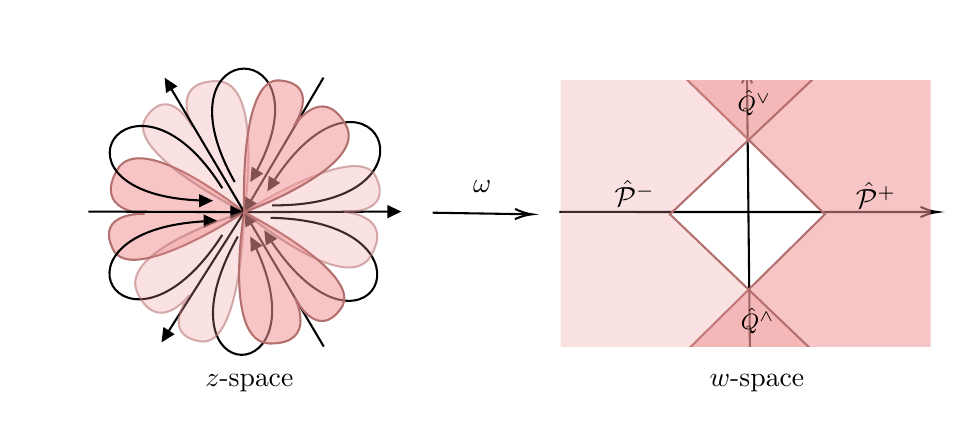
\begin{tikzpicture}[x=0.75pt,y=0.75pt,yscale=-0.75,xscale=0.75]
%uncomment if require: \path (0,286); %set diagram left start at 0, and has height of 286

%Shape: Regular Polygon [id:dp057437658287642135] 
\draw  [color={rgb, 255:red, 180; green, 111; blue, 111 }  ,draw opacity=1 ][fill={rgb, 255:red, 240; green, 149; blue, 149 }  ,fill opacity=0.55 ] (114.98,118.73) .. controls (114.98,118.73) and (82,117.27) .. (97.38,90.48) .. controls (112.76,63.7) and (179,117.64) .. (179,117.64) .. controls (179,117.64) and (106.31,165.61) .. (94.65,141.45) .. controls (83,117.28) and (114.98,118.73) .. (114.98,118.73) -- cycle ;
%Shape: Regular Polygon [id:dp12933226822826427] 
\draw  [color={rgb, 255:red, 180; green, 111; blue, 111 }  ,draw opacity=0.55 ][fill={rgb, 255:red, 240; green, 149; blue, 149 }  ,fill opacity=0.27 ] (145.77,62.9) .. controls (145.77,62.9) and (130.41,33.68) .. (161.29,33.46) .. controls (192.18,33.23) and (179,117.64) .. (179,117.64) .. controls (179,117.64) and (100.92,79.06) .. (115.91,56.81) .. controls (130.9,34.55) and (145.77,62.9) .. (145.77,62.9) -- cycle ;
%Straight Lines [id:da7014467597216401] 
\draw    (179,117.64) -- (276.9,117.29) ;
\draw [shift={(279.9,117.28)}, rotate = 539.79] [fill={rgb, 255:red, 0; green, 0; blue, 0 }  ][line width=0.08]  [draw opacity=0] (8.93,-4.29) -- (0,0) -- (8.93,4.29) -- cycle    ;
%Straight Lines [id:da7937079638414151] 
\draw    (179,117.64) -- (129.43,33.86) ;
\draw [shift={(127.9,31.28)}, rotate = 419.39] [fill={rgb, 255:red, 0; green, 0; blue, 0 }  ][line width=0.08]  [draw opacity=0] (8.93,-4.29) -- (0,0) -- (8.93,4.29) -- cycle    ;
%Straight Lines [id:da5652322657720215] 
\draw    (179,117.64) -- (127.51,198.74) ;
\draw [shift={(125.9,201.28)}, rotate = 302.40999999999997] [fill={rgb, 255:red, 0; green, 0; blue, 0 }  ][line width=0.08]  [draw opacity=0] (8.93,-4.29) -- (0,0) -- (8.93,4.29) -- cycle    ;
%Straight Lines [id:da49795176320656886] 
\draw    (229.9,31.28) -- (180.52,115.05) ;
\draw [shift={(179,117.64)}, rotate = 300.51] [fill={rgb, 255:red, 0; green, 0; blue, 0 }  ][line width=0.08]  [draw opacity=0] (8.93,-4.29) -- (0,0) -- (8.93,4.29) -- cycle    ;
%Straight Lines [id:da9443327330326834] 
\draw    (78.9,117.28) -- (176,117.63) ;
\draw [shift={(179,117.64)}, rotate = 180.21] [fill={rgb, 255:red, 0; green, 0; blue, 0 }  ][line width=0.08]  [draw opacity=0] (8.93,-4.29) -- (0,0) -- (8.93,4.29) -- cycle    ;
%Straight Lines [id:da7066291127526734] 
\draw    (230.1,204) -- (180.53,120.22) ;
\draw [shift={(179,117.64)}, rotate = 419.39] [fill={rgb, 255:red, 0; green, 0; blue, 0 }  ][line width=0.08]  [draw opacity=0] (8.93,-4.29) -- (0,0) -- (8.93,4.29) -- cycle    ;
%Curve Lines [id:da8961728852679585] 
\draw    (196.9,113.28) .. controls (317.29,114.27) and (257.51,-0.19) .. (194.84,102.71) ;
\draw [shift={(193.9,104.28)}, rotate = 300.82] [fill={rgb, 255:red, 0; green, 0; blue, 0 }  ][line width=0.08]  [draw opacity=0] (8.93,-4.29) -- (0,0) -- (8.93,4.29) -- cycle    ;
%Curve Lines [id:da6878104068351576] 
\draw    (172.9,98.28) .. controls (118.17,1.15) and (239.67,1.65) .. (183.76,96.83) ;
\draw [shift={(182.9,98.28)}, rotate = 300.98] [fill={rgb, 255:red, 0; green, 0; blue, 0 }  ][line width=0.08]  [draw opacity=0] (8.93,-4.29) -- (0,0) -- (8.93,4.29) -- cycle    ;
%Curve Lines [id:da6213553894464128] 
\draw    (164.9,102.28) .. controls (106.19,8.13) and (40.56,109.63) .. (157.13,110.27) ;
\draw [shift={(158.9,110.28)}, rotate = 539.81] [fill={rgb, 255:red, 0; green, 0; blue, 0 }  ][line width=0.08]  [draw opacity=0] (8.93,-4.29) -- (0,0) -- (8.93,4.29) -- cycle    ;
%Curve Lines [id:da5023612601796306] 
\draw    (164.9,132.28) .. controls (102.21,229.17) and (41.51,125.7) .. (160.1,123.3) ;
\draw [shift={(161.9,123.28)}, rotate = 539.3399999999999] [fill={rgb, 255:red, 0; green, 0; blue, 0 }  ][line width=0.08]  [draw opacity=0] (8.93,-4.29) -- (0,0) -- (8.93,4.29) -- cycle    ;
%Curve Lines [id:da5020349766396639] 
\draw    (174.9,133.28) .. controls (118.18,234.15) and (234.72,234.66) .. (183.68,134.79) ;
\draw [shift={(182.9,133.28)}, rotate = 422.4] [fill={rgb, 255:red, 0; green, 0; blue, 0 }  ][line width=0.08]  [draw opacity=0] (8.93,-4.29) -- (0,0) -- (8.93,4.29) -- cycle    ;
%Curve Lines [id:da4534345213536044] 
\draw    (195.9,121.28) .. controls (314.3,123.65) and (256.49,233.55) .. (192.86,130.84) ;
\draw [shift={(191.9,129.28)}, rotate = 418.73] [fill={rgb, 255:red, 0; green, 0; blue, 0 }  ][line width=0.08]  [draw opacity=0] (8.93,-4.29) -- (0,0) -- (8.93,4.29) -- cycle    ;
%Shape: Regular Polygon [id:dp7606065427728967] 
\draw  [color={rgb, 255:red, 180; green, 111; blue, 111 }  ,draw opacity=0.55 ][fill={rgb, 255:red, 240; green, 149; blue, 149 }  ,fill opacity=0.27 ] (143.66,171.03) .. controls (143.66,171.03) and (123.78,197.39) .. (110.41,169.55) .. controls (97.03,141.71) and (179,117.64) .. (179,117.64) .. controls (179,117.64) and (177.4,204.71) .. (150.88,200.64) .. controls (124.36,196.57) and (143.66,171.03) .. (143.66,171.03) -- cycle ;
%Shape: Regular Polygon [id:dp10499407073436307] 
\draw  [color={rgb, 255:red, 180; green, 111; blue, 111 }  ,draw opacity=1 ][fill={rgb, 255:red, 240; green, 149; blue, 149 }  ,fill opacity=0.55 ] (211.54,172.79) .. controls (211.54,172.79) and (226.53,202.2) .. (195.65,202.03) .. controls (164.76,201.87) and (179,117.64) .. (179,117.64) .. controls (179,117.64) and (256.59,157.19) .. (241.32,179.26) .. controls (226.05,201.32) and (211.54,172.79) .. (211.54,172.79) -- cycle ;
%Shape: Regular Polygon [id:dp8804803151402205] 
\draw  [color={rgb, 255:red, 180; green, 111; blue, 111 }  ,draw opacity=0.55 ][fill={rgb, 255:red, 240; green, 149; blue, 149 }  ,fill opacity=0.27 ] (243.03,117.46) .. controls (243.03,117.46) and (275.99,119.4) .. (260.23,145.96) .. controls (244.47,172.52) and (179,117.64) .. (179,117.64) .. controls (179,117.64) and (252.36,70.71) .. (263.68,95.04) .. controls (274.99,119.37) and (243.03,117.46) .. (243.03,117.46) -- cycle ;
%Shape: Regular Polygon [id:dp31635047471359634] 
\draw  [color={rgb, 255:red, 180; green, 111; blue, 111 }  ,draw opacity=1 ][fill={rgb, 255:red, 240; green, 149; blue, 149 }  ,fill opacity=0.55 ] (210.97,62.16) .. controls (210.97,62.16) and (229.18,34.62) .. (244.25,61.58) .. controls (259.32,88.54) and (179,117.64) .. (179,117.64) .. controls (179,117.64) and (175.2,30.63) .. (201.93,33.05) .. controls (228.65,35.47) and (210.97,62.16) .. (210.97,62.16) -- cycle ;
%Straight Lines [id:da8740701060140308] 
\draw    (503.9,211.04) -- (501.92,26.04) ;
\draw [shift={(501.9,24.04)}, rotate = 449.39] [color={rgb, 255:red, 0; green, 0; blue, 0 }  ][line width=0.75]    (10.93,-3.29) .. controls (6.95,-1.4) and (3.31,-0.3) .. (0,0) .. controls (3.31,0.3) and (6.95,1.4) .. (10.93,3.29)   ;
%Straight Lines [id:da9217871639595665] 
\draw    (381.4,117.52) -- (622.4,117.56) ;
\draw [shift={(624.4,117.56)}, rotate = 180.01] [color={rgb, 255:red, 0; green, 0; blue, 0 }  ][line width=0.75]    (10.93,-3.29) .. controls (6.95,-1.4) and (3.31,-0.3) .. (0,0) .. controls (3.31,0.3) and (6.95,1.4) .. (10.93,3.29)   ;
%Straight Lines [id:da17434601685188045] 
\draw [color={rgb, 255:red, 180; green, 111; blue, 111 }  ,draw opacity=1 ][fill={rgb, 255:red, 240; green, 149; blue, 149 }  ,fill opacity=0.55 ]   (619.9,209.04) -- (461.9,208.04) -- (552,119) -- (461.9,31.04) -- (619.9,29.04) ;
%Shape: Rectangle [id:dp9982084508684994] 
\draw  [draw opacity=0][fill={rgb, 255:red, 255; green, 255; blue, 255 }  ,fill opacity=1 ] (445,6) -- (625.9,6) -- (625.9,33.04) -- (445,33.04) -- cycle ;
%Shape: Rectangle [id:dp261442729168085] 
\draw  [draw opacity=0][fill={rgb, 255:red, 255; green, 255; blue, 255 }  ,fill opacity=1 ] (452,204) -- (632.9,204) -- (632.9,231.04) -- (452,231.04) -- cycle ;
%Straight Lines [id:da4321981089701783] 
\draw [color={rgb, 255:red, 180; green, 111; blue, 111 }  ,draw opacity=1 ][fill={rgb, 255:red, 240; green, 149; blue, 149 }  ,fill opacity=0.27 ]   (382.33,209.04) -- (545.54,208.04) -- (452.47,119) -- (545.54,31.04) -- (446.39,29.83) -- (382.33,29.04) ;
%Shape: Rectangle [id:dp1675953452553458] 
\draw  [draw opacity=0][fill={rgb, 255:red, 255; green, 255; blue, 255 }  ,fill opacity=1 ] (563,6) -- (376.13,6) -- (376.13,33.04) -- (563,33.04) -- cycle ;
%Shape: Rectangle [id:dp26924443276601817] 
\draw  [draw opacity=0][fill={rgb, 255:red, 255; green, 255; blue, 255 }  ,fill opacity=1 ] (555.77,204) -- (368.9,204) -- (368.9,231.04) -- (555.77,231.04) -- cycle ;
%Straight Lines [id:da5027547130138361] 
\draw    (300,118) -- (361.9,119.01) ;
\draw [shift={(363.9,119.04)}, rotate = 180.93] [color={rgb, 255:red, 0; green, 0; blue, 0 }  ][line width=0.75]    (10.93,-3.29) .. controls (6.95,-1.4) and (3.31,-0.3) .. (0,0) .. controls (3.31,0.3) and (6.95,1.4) .. (10.93,3.29)   ;

% Text Node
\draw (152,220) node [anchor=north west][inner sep=0.75pt]   [align=left] {$\displaystyle z$-space};
% Text Node
\draw (476,220) node [anchor=north west][inner sep=0.75pt]   [align=left] {$\displaystyle w$-space};
% Text Node
\draw (570,96.4) node [anchor=north west][inner sep=0.75pt]    {$\hat{\mathcal{P}}^{+}$};
% Text Node
\draw (415,95.4) node [anchor=north west][inner sep=0.75pt]    {$\hat{\mathcal{P}}^{-}$};
% Text Node
\draw (494,37.4) node [anchor=north west][inner sep=0.75pt]  [font=\footnotesize]  {$\hat{Q}^{\lor }$};
% Text Node
\draw (496,177.4) node [anchor=north west][inner sep=0.75pt]  [font=\footnotesize]  {$\hat{Q}^{\land }$};
% Text Node
\draw (324,95.4) node [anchor=north west][inner sep=0.75pt]    {$\omega $};


\end{tikzpicture}

    \caption{Illustration of the petals constructed in Theorem~\ref{thm:flower}. Notice the shape of the petals -- can you find an equation for them?}
\end{figure}

\subsection{Abel Linearization}

We now start to think about constructing a linearization for a holomorphic function near a parabolic fixed point. Our earlier experience with the Koenigs linearization might suggest a linearization of the form $\phi(\zeta)=\zeta$, but this is obviously absurd: it would require identifying points that ought not be identified. 

Instead, we are inspired by the structure of a petal, which comes with some notion of ``direction'' defined on it. One may imagine rearranging the petal so that application of $f$ is just adding 1, i.e. consider (where $\zeta=T(z)$, $\phi=T\circ f\circ T^{-1}$) a linearization of the form $\phi(\zeta)=\zeta+1$. One may imagine that this would be closely related to the quotient $\mathcal{P}/f$. 

\begin{thm}[Parabolic linearization theorem]
    \label{thm:linear}
    Given an attracting or repelling petal $\mathcal{P}$, there exists a unique (up to composition on the left with translation) conformal embedding $T:\mathcal{P}\to\mathbb{C}$ called a Fatou co-ordinate on $\mathcal{P}$ such that, for all $z\in\mathcal{P}\cup f^{-1}(\mathcal{P})$, we have:
    \begin{equation*}
        T(f(z))=T(z)+1
    \end{equation*}
\end{thm}

Here's an idea to construct this $T$: recall how in $w$-space, we have $\hat{f}(w) = w + 1 + o(1)$. Well, it is not exact, but as you keep applying $\hat{f}$, $|w|\to\infty$ and it becomes more and more exact. So we may consider representing $w$ by some $\hat{f}^n(w)$ for large $n$. More precisely, we'd need to set some base point and replace $w\mapsto \hat{f}^n(w)-\hat{f}^n(w_O)$.

\begin{lem}
    \label{lem:That}
    Where $\hat{\mathcal{P}}_R=\{w\mid \mathrm{Re}(w) > R\}$ for some $R$, and $\hat{f}:\hat{\mathcal{P}}_R\to\hat{\mathcal{P}}_R$ is an injective holomorphic function satisfying the following inequalities, for constants $c, \varepsilon > 0$:
    \begin{equation*}
        \mathrm{Re}(\hat{f}(w)) > \mathrm{Re}(w) + 1/2
    \end{equation*}
    \begin{equation*}
        \left|\hat{f}(w+1)-(w+1)\right| \le c/|w|^\varepsilon
    \end{equation*}
    Then, where $w_O$ is some arbitrary base point in $\hat{\mathcal{P}}_R$, the following sequence of functions: 
    \begin{equation*}
        \hat{T}_n(w)=\hat{f}^n(w)-\hat{f}^n(w_O)
    \end{equation*}
    Converges locally uniformly to a bi-holomorphic map $\hat{T}:\hat{\mathcal{P}}_R\to U\subset \mathbb{C}$ that satisfies $T(\hat{f}(w))=T(w)+1$.
\end{lem}
\begin{proof}
    The ratio $\hat{T}_n(w)/\hat{T}_{n-1}(w)$ is relevant for questions of convergence, and is seen to be the average slope of $\hat{f}$ along the line segment from $\hat{f}^n(w_O)$ to $\hat{f}^n(w)$. Well, when $|w|\ge 2S \ge 2R$, the function $\hat{f}(w)-(1+w)$ transforms $\mathbb{D}_S(w)\mapsto \mathbb{D}_{c/S^\varepsilon}(0)$, so by the Cauchy derivative estimate:
    \begin{equation*}
        \left|\hat{f}'(w)-1\right|<c/S^{1+\varepsilon}
    \end{equation*}
    The same bound thus applies on the average slope between $w_1, w_2\in \hat{\mathcal{P}}_{2S}$:
    \begin{equation*}
        \left|\frac{\hat{f}(w_2)-\hat{f}(w_1)}{w_2-w_1}-1\right|\le \frac{c}{S^{1+\varepsilon}} 
    \end{equation*}
    Since $\mathrm{Re}(\hat{f}^n(w))>n/2$, we can write for all $n\ge 1$, $c'=2^{1+\varepsilon} c$:
    \begin{equation}
        \label{eq:ratbd1}
        \left|\frac{\hat{T}_n(w)}{\hat{T}_{n-1}(w)} - 1\right|\le \frac{c'}{n^{1+\varepsilon}}
    \end{equation}    
    \begin{equation*}
        1-\frac{c'}{n^{1+\varepsilon}} \le 
        \left|\frac{\hat{T}_n(w)}{\hat{T}_{n-1}(w)}\right| \le 1+\frac{c'}{n^{1+\varepsilon}}
    \end{equation*}    
    Noting that $K=\prod\left(1+c'/n^{1+\varepsilon}\right)$ is finite:
    \begin{equation}
        \label{eq:bd}
        \left|\hat{T}_n(w)\right|\le K\, |w-w_O|
    \end{equation}
    Considering Eq.~\ref{eq:bd} for $n\mapsto n-1$ and multiplying by Eq.~\ref{eq:ratbd1},
    \begin{equation}
        \label{eq:difbd}
        \left|\hat{T}_n(w)-\hat{T}_{n-1}(w)\right|\le Kc'|w-w_O|/n^{1+\varepsilon} 
    \end{equation}
    If we sum Eq.~\ref{eq:difbd}, it is clear that the sum of the right-hand-side converges absolutely, thus the sum:
    \begin{equation*}
        \hat{T}_0(w)+\sum_{n=1}^\infty \left({\hat{T}_n(w)-\hat{T}_{n-1}(w)}\right)
    \end{equation*}
    Is absolutely convergent, therefore the desired limit exists $\forall w\in\hat{\mathcal{P}}_{2R}$: 
    \begin{equation*}
        \hat{T}(w)=\lim_{n\to\infty}\hat{T}_n(w)
    \end{equation*}
    From Eq.~\ref{eq:difbd}, we see that $\hat{T}_n(w)/|w-w_O|$ converges uniformly to $\hat{T}(w)/|w-w_O|$ (because the error does not depend on $w$), which shows that the limiting function $T(w)$ is holomorphic, and the injectivity of $T$ follows immediately from the injectivity of $f$ and injectivity of the uniform limit of injective functions. 
\end{proof}

\begin{proof}[Proof of Theorem~\ref{thm:linear} -- Existence]
    In the case where the petal is $\mathcal{P}_R = \omega^{-1}(\hat{P}_R)$, the function $T=\hat{T}\circ\omega$ suffices, with $\hat{T}$ defined as in Lemma~\ref{lem:That} and $\omega$ defined as in \ref{thm:arvec-ir}. For an arbitrary petal $\mathcal{P}$: recall that by definition of a petal, any $z\in\mathcal{P}$ must eventually have $f^n(z)\in\mathcal{P}_R$ -- so define $T(z)=\hat{T}\circ\omega\circ f^n(z) - n$.
\end{proof}

For uniqueness, we will need a minor lemma (which you should read after).

\begin{lem}
    \label{lem:strip}
    The union of all integer translations of $U$ as defined in Lemma~\ref{lem:That}, $U+\mathbb{Z}$, is all of $\mathbb{C}$. 
\end{lem}
\begin{proof}
    We wish to show that $\forall w\in\mathbb{C}, \exists m\in\mathbb{Z}, w+m\in U$. Where $S$ is large enough that $\forall w_\cdot\in\hat{\mathcal{P}}_R\cap(\overline{\mathbb{D}}_S(0))^c, |\hat{T}(w_\cdot)-w_\cdot|<|w_\cdot|/3$, choose a $w_\cdot=w+m$ with a sufficiently high real part that $|w_\cdot|>2S$ and $\overline{\mathbb{D}}_{|w_\cdot|/2}(w_\cdot)\subset \hat{\mathcal{P}}_R$. Then for any $w_{\bullet}\in\overline{\mathbb{D}}_{|w_\cdot|/2}(w_\cdot)$, we have $|w_{\bullet}|>S\implies |\hat{T}(w_{\bullet})-w_{\bullet}|<|w_{\bullet}|/3<(3|w_\cdot|/2)/3=|w_\cdot|/2$. Since $|w_\cdot|/2$ is the radius of $\overline{\mathbb{D}}_{|w_\cdot|/2}(w_\cdot)$, we have that for all $w_{\circ}\in\partial\overline{\mathbb{D}}_{|w_\cdot|/2}(w_\cdot), |\hat{T}(w_{\circ})-w_{\circ}| < |w_{\circ}-w_\cdot|$. Then by Rouche's theorem, the function $\hat{T}(w_\bullet)-w_\cdot=(\hat{T}(w_\bullet)-w_\bullet)+(w_\bullet-w_\cdot)$ has the same number of zeroes as $w_\bullet-w_\cdot$, i.e. one, i.e. $\exists w_\bullet$ such that $\hat{T}(w_\bullet)=w_\cdot$. Hence $w_\cdot\in U$.
\end{proof}

\begin{proof}[Proof of Theorem~\ref{thm:linear} -- Uniqueness]
    First consider the case of $\mathcal{P}_R$, as before, and consider some alternative Abel linearization $T': \mathcal{P}_R\to U'$. Then $E=T'\circ T^{-1}$ is a bijection $U\to U'$ that preserves the ``plus one'' structure, i.e. $E(w+1)=E(w)+1$. As the union of integer translations of $U$ is all of $\mathbb{C}$, then we could use this property (i.e. through $E(w+n)=E(w)+n$) to define a a bijective map $E:\mathbb{C}\to U'+\mathbb{Z}$. Such a map must be affine, and the only affine maps satisfying $E(w+1)=E(w)+1$ are translations.
\end{proof}

\begin{cor}[Cylinder theorem]
    \label{cor:cyl}
    For any petal $\mathcal{P}$ attracting or repelling, $\mathcal{P}/f$ is conformally isomorphic to the cylinder $\mathbb{C}/\mathbb{Z}$.
\end{cor}

As with the Koenigs linearization, we can also define global linearizations. However, these are not necessarily injective. 
\begin{cor}[Global linearization -- attracting petal]
    Where $\mathcal{P}$ is an attracting petal in the attracting basin $\mathcal{B}$, the Fatou co-ordinate $T:\mathcal{P}\to\mathbb{C}$ extends uniquely to a map $\mathcal{B}\to\mathbb{C}$, still satisfying $T(f(z))=T(z)+1$. 
\end{cor}
\begin{cor}[Global linearization -- repelling petal]
    Where $\mathcal{P}$ is a repelling petal, the inverse map $T^{-1}:T(\mathcal{P})\to\mathcal{P}$ extends uniquely to a map $\mathbb{C}\to\mathbb{C}$, satisfying $f(T^{-1}(w))=T^{-1}(w+1)$. 
\end{cor}

\end{document}
